\section{Vista de datos}
La vista de datos se muestra como una adicional al modelo 4+1 con el que se está trabajando, en esta vista se muestra el modelo relacional de la base de datos tal como se puede observar en la Figura \ref{fig:Entidad}.
\subsection{Diagrama relacional}

\begin{figure}[H]
	\begin{center}
		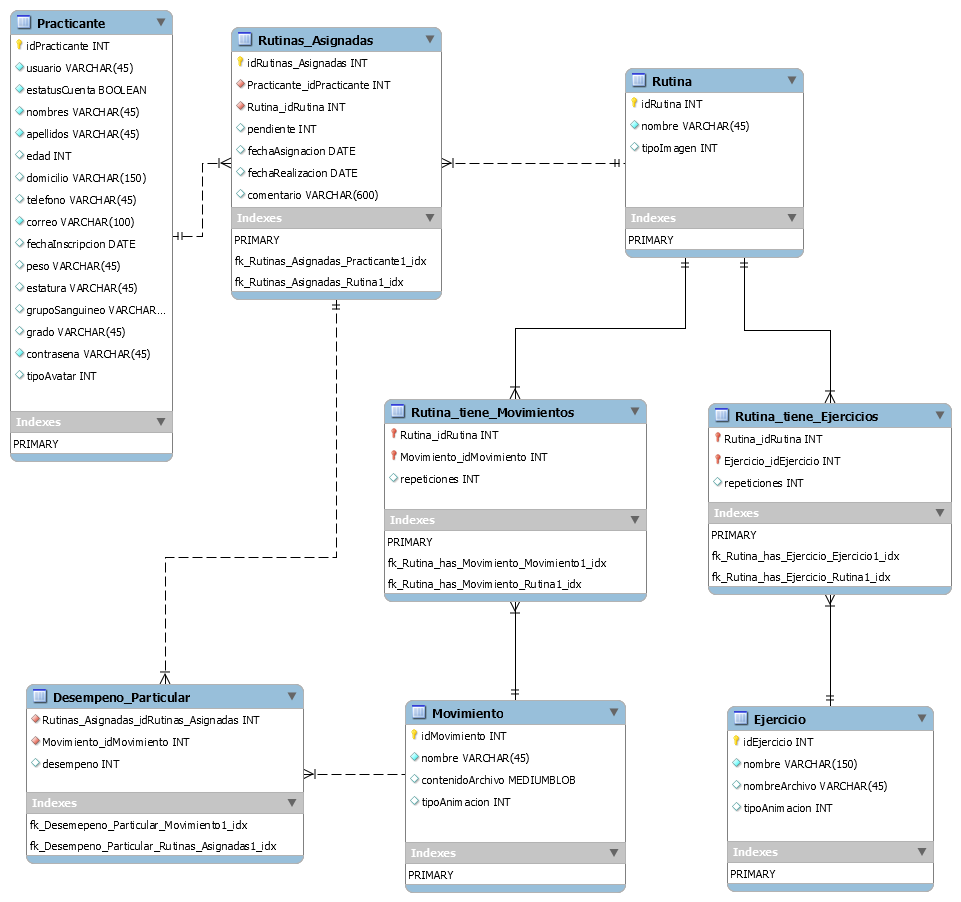
\includegraphics[scale=0.5]{./Figuras/Arquitectura/Modelo_relacional}
	\end{center}
	\caption{Modelo relacional}
	\label{fig:Entidad}
\end{figure}

\subsection{Diccionario de datos}
\label{sec:diccionario}

El diccionario de datos precisa los datos de entrada, salida, componentes de movimientos y rutinas así como detalles de las relaciones entre cada uno de ellos que se manejan en la herramienta.\\[0.5cm]
\textbf{Nombre de la base de datos: }KarateTraining \hspace{0.5cm}\textbf{Fecha de creación: }Abril del 2015.\\[0.25cm]
\textbf{Descripción: }Base de datos de la herramienta KarateTraining que contiene la información de gestión de practicantes, movimientos, rutinas y desempeño.

% Practicante
%--------------------------------------------------------------------------------------------------------
\begin{table}[H]
\centering
\resizebox{17cm}{!}{	%Para redimensionar la tabla
\begin{tabular}{| c | l | l | c | p{8cm}|}
\hline
\rowcolor[rgb]{0.529412, 0.807843, 0.980392}\multicolumn{5}{|l|}{ \textbf{Practicante} }\\
\hline
\textbf{Llave} &  \textbf{Campo} & \textbf{Tipo} & \textbf{Tamaño} & \textbf{Descripción}\\
\hline
PK & idPracticante & Numérico & 11 & Identificador único del Practicante.\\
\hline
 & usuario & Carácter & 45 & Nombre de usuario del Practicante.\\
\hline	
 & estatusCuenta & Numérico & 1 & Estatus de la cuenta del Practicante.\\
\hline	
 & nombres & Carácter & 45 & Nombre(s) del Practicante.\\
\hline 
& apellidos & Carácter & 45 & Apellido(s) del Practicante.\\
\hline
 & edad & Numérico & 11 & Edad del Practicante.\\
\hline
 & domicilio & Carácter & 150 & Domicilio del Practicante.\\
\hline
 & correo & Carácter & 100 & Correo electrónico del Practicante.\\
\hline
 & fechaInscripción & Fecha &  & Fecha de inscripción del Practicante en la herramienta.\\
\hline
 & peso & Carácter & 45 & Peso del Practicante.\\
\hline
 & estatura & Carácter & 45 & Estatura del Practicante.\\
\hline
 & grupoSanguíneo & Carácter & 45 & Grupo sanguíneo del del Practicante.\\
\hline
 & grado & Carácter & 45 & Grado de cinta en Karate Do del Practicante.\\
 \hline
 & contrasena & Carácter & 45 & Contraseña del Practicante para iniciar sesión en la herramienta.\\
\hline
 & tipoAvatar & Numérico & 11 & Tipo de avatar del Practicante para la interfaz.\\
\hline
\end{tabular}
}
\caption{Tabla Practicante}
\label{tab:DDPracticante}
\end{table} 

% Ejercicio
%--------------------------------------------------------------------------------------------------------
\begin{table}[H]
\centering
\resizebox{17cm}{!}{	%Para redimensionar la tabla
\begin{tabular}{| c | l | l | c | p{8cm}|}
\hline
\rowcolor[rgb]{0.529412, 0.807843, 0.980392}\multicolumn{5}{|l|}{ \textbf{Ejercicio} }\\
\hline
\textbf{Llave} &  \textbf{Campo} & \textbf{Tipo} & \textbf{Tamaño} & \textbf{Descripción}\\
\hline
PK & idEjercicio & Numérico & 11 & Identificador único de los ejercicios.\\
\hline
 & nombre & Carácter & 150 & Nombre del ejercicio de calentamiento.\\
\hline
 & tipoAnimación & Numérico & 11 & Tipo de animación que se muestra en la interfaz.\\
\hline
\end{tabular}
}
\caption{Tabla Ejercicio}
\label{tab:DDEjercicio}
\end{table}

% Movimiento
%--------------------------------------------------------------------------------------------------------
\begin{table}[H]
\centering
\resizebox{17cm}{!}{	%Para redimensionar la tabla
\begin{tabular}{| c | l | l | c | p{8cm}|}
\hline
\rowcolor[rgb]{0.529412, 0.807843, 0.980392}\multicolumn{5}{|l|}{ \textbf{Movimiento} }\\
\hline
\textbf{Llave} &  \textbf{Campo} & \textbf{Tipo} & \textbf{Tamaño} & \textbf{Descripción}\\
\hline
PK & idEjercicio & Numérico & 11 & Identificador único de los movimientos.\\
\hline
 & nombre & Carácter & 150 & Nombre del movimiento de técnica.\\
\hline
 & contenidoArchivo & Archivo &  & Vector de bytes que almacena el archivo XML con el movimiento capturado.\\
\hline
 & tipoAnimación & Numérico & 11 & Tipo de animación que se muestra en la interfaz.\\
\hline
\end{tabular}
}
\caption{Tabla Movimiento}
\label{tab:DDMovimiento}
\end{table}

% Rutina
%--------------------------------------------------------------------------------------------------------
\begin{table}[H]
\centering
\resizebox{17cm}{!}{	%Para redimensionar la tabla
\begin{tabular}{| c | l | l | c | p{8cm}|}
\hline
\rowcolor[rgb]{0.529412, 0.807843, 0.980392}\multicolumn{5}{|l|}{ \textbf{Rutina} }\\
\hline
\textbf{Llave} &  \textbf{Campo} & \textbf{Tipo} & \textbf{Tamaño} & \textbf{Descripción}\\
\hline
PK & idRutina & Numérico & 11 & Identificador único de las rutinas.\\
\hline
 & nombre & Carácter & 45 & Nombre de la rutina.\\
\hline
 & tipoImagen & Numérico & 11 & Tipo de la imagen alusiva de la rutina.\\
\hline
\end{tabular}
}
\caption{Tabla Rutina}
\label{tab:DDRutina}
\end{table} 

% Rutina tiene ejercicios
%--------------------------------------------------------------------------------------------------------
\begin{table}[H]
\centering
\resizebox{17cm}{!}{	%Para redimensionar la tabla
\begin{tabular}{| c | l | l | c | p{8cm}|}
\hline
\rowcolor[rgb]{0.529412, 0.807843, 0.980392}\multicolumn{5}{|l|}{ \textbf{Rutina\_tiene\_Ejercicios} }\\
\hline
\textbf{Llave} &  \textbf{Campo} & \textbf{Tipo} & \textbf{Tamaño} & \textbf{Descripción}\\
\hline
FK & Rutina\_idRutina & Numérico & 11 & Llave foránea del id de la rutina.\\
\hline
FK & Ejercicio\_idEjercicio & Numérico & 11 & Llave foránea del id del ejercicio.\\
\hline
 & repeticiones & Numérico & 11 & Número de repeticiones por cada ejercicio.\\
\hline
\end{tabular}
}
\caption{Tabla Rutina\_tiene\_Ejercicios}
\label{tab:DDRutina_tiene_Ejercicios}
\end{table} 

% Rutina tiene movimientos
%--------------------------------------------------------------------------------------------------------
\begin{table}[H]
\centering
\resizebox{17cm}{!}{	%Para redimensionar la tabla
\begin{tabular}{| c | l | l | c | p{8cm}|}
\hline
\rowcolor[rgb]{0.529412, 0.807843, 0.980392}\multicolumn{5}{|l|}{ \textbf{Rutina\_tiene\_Movimientos} }\\
\hline
\textbf{Llave} &  \textbf{Campo} & \textbf{Tipo} & \textbf{Tamaño} & \textbf{Descripción}\\
\hline
FK & Rutina\_idRutina & Numérico & 11 & Llave foránea del id de la rutina.\\
\hline
FK & Movimiento\_idMovimiento & Numérico & 11 & Llave foránea del id del movimiento.\\
\hline
 & repeticiones & Numérico & 11 & Número de repeticiones por cada movimiento.\\
\hline
\end{tabular}
}
\caption{Tabla Rutina\_tiene\_Movimientos}
\label{tab:DDRutina_tiene_Movimientos}
\end{table} 

% Rutinas asignadas
%--------------------------------------------------------------------------------------------------------
\begin{table}[H]
\centering
\resizebox{17cm}{!}{	%Para redimensionar la tabla
\begin{tabular}{| c | l | l | c | p{8cm}|}
\hline
\rowcolor[rgb]{0.529412, 0.807843, 0.980392}\multicolumn{5}{|l|}{ \textbf{Rutinas\_Asignadas} }\\
\hline
\textbf{Llave} &  \textbf{Campo} & \textbf{Tipo} & \textbf{Tamaño} & \textbf{Descripción}\\
\hline
PK & idRutinas\_Asignadas & Numérico & 11 & Identificador único de las rutinas asignadas.\\
\hline
FK & Practicante\_idPracticante & Numérico & 11 & Llave foránea del id del Practicante.\\
\hline
FK & Rutina\_idRutina & Numérico & 11 & Llave foránea del id de la rutina.\\
\hline
 & pendiente & Numérico & 11 & Estado de realización de una rutina.\\
\hline
 & fechaAsignacion & Fecha &  & Fecha de asignación de una rutina.\\
\hline
 & fechaRealizacion & Fecha &  & Fecha de realización de una rutina.\\
\hline
 & comentario & Carácter & 600 & Comentario realizado por el Entrenador.\\
\hline
\end{tabular}
}
\caption{Tabla Rutinas\_Asignadas}
\label{tab:DDRutinas_Asignadas}
\end{table} 

% Desempeño particular
%--------------------------------------------------------------------------------------------------------
\begin{table}[H]
\centering
\resizebox{17cm}{!}{	%Para redimensionar la tabla
\begin{tabular}{| c | l | l | c | p{8cm}|}
\hline
\rowcolor[rgb]{0.529412, 0.807843, 0.980392}\multicolumn{5}{|l|}{ \textbf{Desempeno\_Particular} }\\
\hline
\textbf{Llave} &  \textbf{Campo} & \textbf{Tipo} & \textbf{Tamaño} & \textbf{Descripción}\\
\hline
FK & Rutinas\_Asignadas\_idRutinas\_Asignadas & Numérico & 11 & Llave foránea del id de las rutinas asignadas.\\
\hline
FK & Movimiento\_idMovimiento & Numérico & 11 & Llave foránea del id del movimiento.\\
\hline
 & desempeno & Numérico & 11 & Desempeño obtenido por cada movimiento realizado.\\
\hline
\end{tabular}
}
\caption{Tabla Desempeno\_Particular}
\label{tab:DDDesempeno_Particular}
\end{table} 

\clearpage